

\documentclass[tikz,border=10pt]{standalone}
\usetikzlibrary{arrows.meta,positioning}

\begin{document}
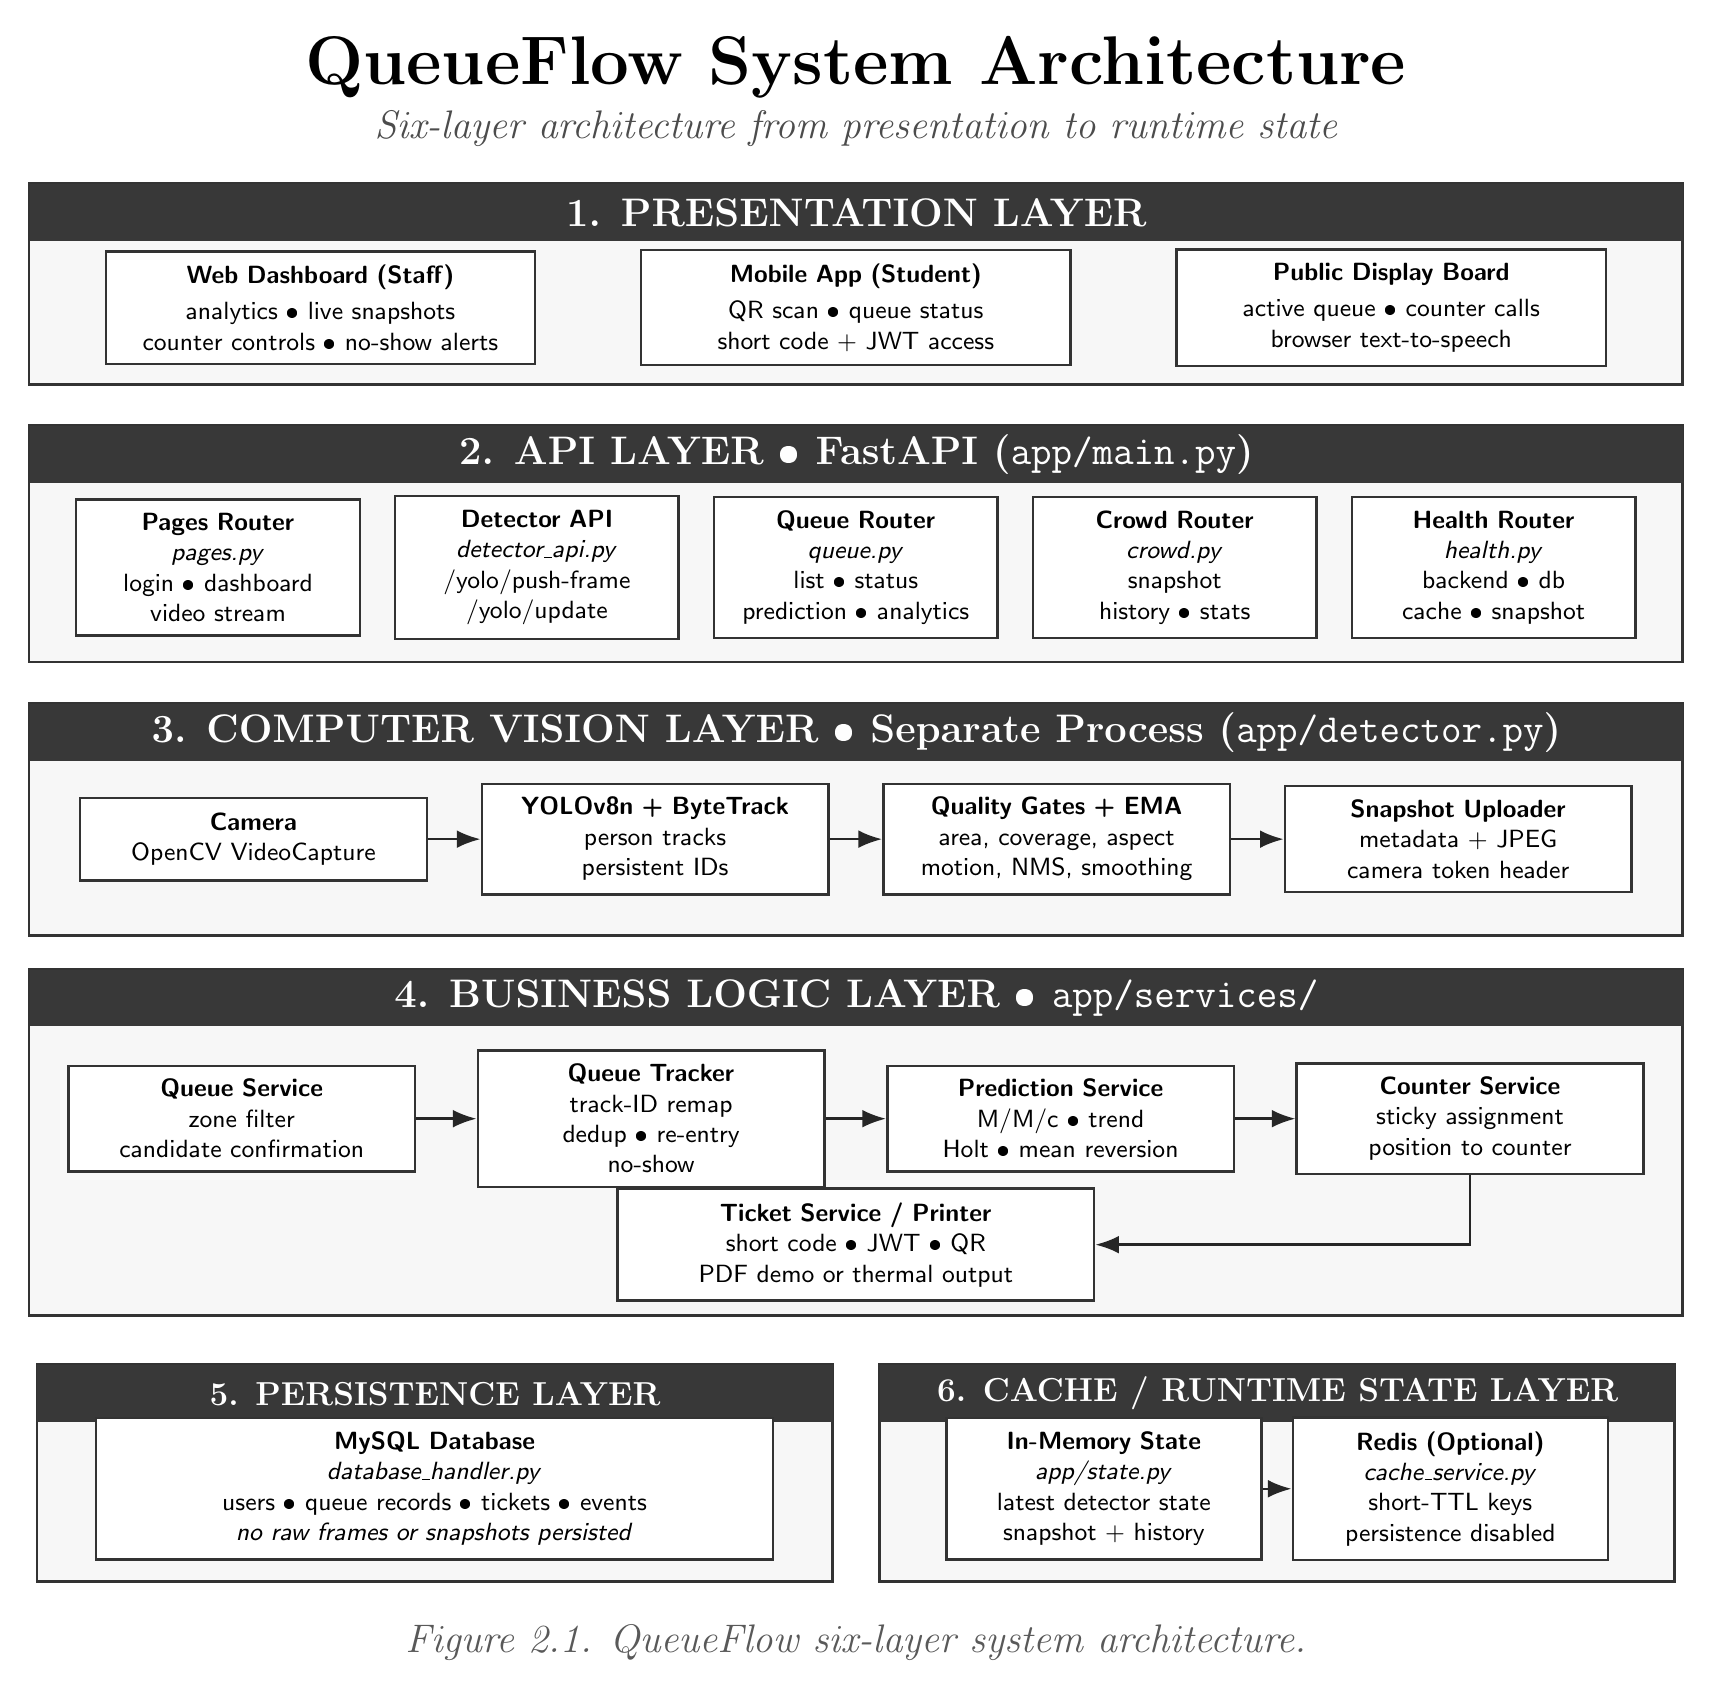
\begin{tikzpicture}[
  font=\sffamily,
  layer/.style={draw=black!80, line width=1pt, fill=black!3,
    minimum width=21.0cm, minimum height=2.25cm},
  header/.style={fill=black!78, text=white, font=\bfseries\Large,
    minimum width=21.0cm, minimum height=0.72cm, anchor=north west,
    align=center, inner sep=0pt},
  halfheader/.style={header, font=\bfseries\large},
  box/.style={draw=black!80, line width=0.9pt, fill=white, align=center,
    minimum height=1.05cm, inner sep=5pt, font=\sffamily\small},
  widebox/.style={box, text width=5.1cm},
  medbox/.style={box, text width=4.05cm},
  smallbox/.style={box, text width=3.25cm},
  arrow/.style={-{Latex[length=3mm]}, line width=0.9pt, black!85}
]

\node[font=\bfseries\Huge] at (0,0) {QueueFlow System Architecture};
\node[font=\itshape\Large, text=black!70] at (0,-0.78)
  {Six-layer architecture from presentation to runtime state};

% Layer 1
\node[layer, minimum height=2.55cm] (presentation) at (0,-2.75) {};
\node[header] at ([xshift=-10.5cm,yshift=1.275cm]presentation.center)
  {1. PRESENTATION LAYER};
\node[widebox] (dash) at (-6.8,-3.05)
  {\textbf{Web Dashboard (Staff)}\\[2pt]
   analytics \textbullet{} live snapshots\\
   counter controls \textbullet{} no-show alerts};
\node[widebox] (mobile) at (0,-3.05)
  {\textbf{Mobile App (Student)}\\[2pt]
   QR scan \textbullet{} queue status\\
   short code + JWT access};
\node[widebox] (display) at (6.8,-3.05)
  {\textbf{Public Display Board}\\[2pt]
   active queue \textbullet{} counter calls\\
   browser text-to-speech};

% Layer 2
\node[layer, minimum height=3.0cm] (api) at (0,-6.05) {};
\node[header] at ([xshift=-10.5cm,yshift=1.5cm]api.center)
  {2. API LAYER \textbullet{} FastAPI (\texttt{app/main.py})};
\node[smallbox] (pages) at (-8.1,-6.35)
  {\textbf{Pages Router}\\\textit{pages.py}\\login \textbullet{} dashboard\\video stream};
\node[smallbox] (detapi) at (-4.05,-6.35)
  {\textbf{Detector API}\\\textit{detector\_api.py}\\/yolo/push-frame\\/yolo/update};
\node[smallbox] (queueapi) at (0,-6.35)
  {\textbf{Queue Router}\\\textit{queue.py}\\list \textbullet{} status\\prediction \textbullet{} analytics};
\node[smallbox] (crowd) at (4.05,-6.35)
  {\textbf{Crowd Router}\\\textit{crowd.py}\\snapshot\\history \textbullet{} stats};
\node[smallbox] (health) at (8.1,-6.35)
  {\textbf{Health Router}\\\textit{health.py}\\backend \textbullet{} db\\cache \textbullet{} snapshot};

% Layer 3
\node[layer, minimum height=2.95cm] (cv) at (0,-9.55) {};
\node[header] at ([xshift=-10.5cm,yshift=1.475cm]cv.center)
  {3. COMPUTER VISION LAYER \textbullet{} Separate Process (\texttt{app/detector.py})};
\node[medbox] (camera) at (-7.65,-9.8)
  {\textbf{Camera}\\OpenCV VideoCapture};
\node[medbox] (yolo) at (-2.55,-9.8)
  {\textbf{YOLOv8n + ByteTrack}\\person tracks\\persistent IDs};
\node[medbox] (gates) at (2.55,-9.8)
  {\textbf{Quality Gates + EMA}\\area, coverage, aspect\\motion, NMS, smoothing};
\node[medbox] (upload) at (7.65,-9.8)
  {\textbf{Snapshot Uploader}\\metadata + JPEG\\camera token header};

% Layer 4
\node[layer, minimum height=4.4cm] (logic) at (0,-13.65) {};
\node[header] at ([xshift=-10.5cm,yshift=2.2cm]logic.center)
  {4. BUSINESS LOGIC LAYER \textbullet{} \texttt{app/services/}};
\node[medbox] (qsvc) at (-7.8,-13.35)
  {\textbf{Queue Service}\\zone filter\\candidate confirmation};
\node[medbox] (tracker) at (-2.6,-13.35)
  {\textbf{Queue Tracker}\\track-ID remap\\dedup \textbullet{} re-entry\\no-show};
\node[medbox] (pred) at (2.6,-13.35)
  {\textbf{Prediction Service}\\M/M/c \textbullet{} trend\\Holt \textbullet{} mean reversion};
\node[medbox] (counter) at (7.8,-13.35)
  {\textbf{Counter Service}\\sticky assignment\\position to counter};
\node[widebox, text width=5.7cm] (ticket) at (0,-14.95)
  {\textbf{Ticket Service / Printer}\\short code \textbullet{} JWT \textbullet{} QR\\PDF demo or thermal output};

% Layer 5 and 6
\node[layer, minimum width=10.1cm, minimum height=2.75cm] (persist) at (-5.35,-17.85) {};
\node[halfheader, minimum width=10.1cm] at ([xshift=-5.05cm,yshift=1.375cm]persist.center)
  {5. PERSISTENCE LAYER};
\node[box, text width=8.25cm] (mysql) at (-5.35,-18.05)
  {\textbf{MySQL Database}\\\textit{database\_handler.py}\\users \textbullet{} queue records \textbullet{} tickets \textbullet{} events\\\textit{no raw frames or snapshots persisted}};

\node[layer, minimum width=10.1cm, minimum height=2.75cm] (runtime) at (5.35,-17.85) {};
\node[halfheader, minimum width=10.1cm] at ([xshift=-5.05cm,yshift=1.375cm]runtime.center)
  {6. CACHE / RUNTIME STATE LAYER};
\node[box, text width=3.65cm] (state) at (3.15,-18.05)
  {\textbf{In-Memory State}\\\textit{app/state.py}\\latest detector state\\snapshot + history};
\node[box, text width=3.65cm] (redis) at (7.55,-18.05)
  {\textbf{Redis (Optional)}\\\textit{cache\_service.py}\\short-TTL keys\\persistence disabled};

% Arrows
\draw[arrow] (camera) -- (yolo);
\draw[arrow] (yolo) -- (gates);
\draw[arrow] (gates) -- (upload);
\draw[arrow] (qsvc) -- (tracker);
\draw[arrow] (tracker) -- (pred);
\draw[arrow] (pred) -- (counter);
\draw[arrow] (counter.south) |- (ticket.east);
\draw[arrow] (state) -- (redis);

\node[font=\itshape\Large, text=black!65] at (0,-20.0)
  {Figure 2.1. QueueFlow six-layer system architecture.};
\end{tikzpicture}
\end{document}
